\scanpage{5}
\[
\operatorname{réal}(S,A,R)\lhook\joinrel\longrightarrow E
\]
such that the image of an arc is a segment.

\uline{Proposition} For a finite graph to admit a rectilinear geometric realization, (in a suitable vector space over $\mathbb{R}$) it is necessary and sufficient that it \deleted{\unsure{has|is}} be strict -- and then it admits a rectilinear realization in $\mathbb{R}^{3}$. More precisely, if $S\hookrightarrow\deleted{\unsure{\mathbb{R}^{3}|R^{3}}}E$ \inserted{$(\simeq\mathbb{R}^{3},\ \unsure{v.a.|v.ex.})$} is an immersion such that
\figure{\begin{tikzpicture}[x=.025cm,y=.025cm]
\draw[line width=.7pt] (0,0)--(31,34);
\draw[line width=.3pt] (34,38)--(60,66);
\draw (0,0) circle (1.5);
\fill (31,34) circle (1.45);
\fill (60,66) circle (1.2);
\end{tikzpicture}}
\[
\forall x,y\in S\quad x\ne y,\quad \text{one has}\quad
\deleted{\unsure{\{|\exists}}
\underbrace{\overline{x,y}}_{\substack{\text{segment}\\\text{joining}\\x\ \text{to}\ y}}\cap S=\{x,y\},
\]
\inserted{(i.e. three \inserted{distinct} points never collinear)}
\inserted{and $\forall x,y,z,t$ distinct, $(\overline{x,y})\cap(\overline{z,t})=\varnothing$}

$\exists 1$ rectilinear geometric realization $\unsure{\operatorname{réll}|\operatorname{réel}|\operatorname{réal}}(S,A,R)\lhook\joinrel-E$ which f \unsure{extends|extends\textsuperscript{?}}\ldots

Connected graph $=$ connected geometric realization $=$ which is not a \deleted{\unsure{union}} ``sum'' of two other graphs $\ne\varnothing$

\uline{NB} Every graph is uniquely a union of connected \inserted{and disjoint} graphs

[ sum graph : $S\amalg S',\quad A\amalg A',\quad R\amalg R'\ \ldots$ ]

% A curved arrow in the left margin leads from NB to the next heading.
\margin{\figure{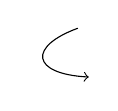
\begin{tikzpicture}[baseline=-.5ex,x=1cm,y=1cm]\draw[->] (.48,.62) .. controls (-.15,.39) and (-.12,.04) .. (.62,0);\end{tikzpicture}}}
\inserted{Multi}polygonal graph \inserted{(or \uline{contour} (combinatorial))}
\[
\bigl[\quad\forall s\in S,\quad\operatorname{card}R\{s\}=2\quad\bigr]
\]

Duality of \deleted{polygonal graphs} contours (combinatorial).

\deleted{\unsure{thus|thus}} the \inserted{\unsure{connected|connected}} components of a \deleted{polygonal graph}\inserted{contour} are \deleted{polygonal.} contours.

Classification of connected \deleted{polygonal graphs}\inserted{contours} $\ne\varnothing$

\uline{Proposition} A connected \deleted{polygonal graph}\inserted{contour} \inserted{$\ne\varnothing$} is known up to isomorphism when one knows $\operatorname{card}S$ ($=\operatorname{card}A$), which is any cardinal \deleted{finite or infinite}
\[
2\le c\le\aleph_{0}
\]
(strict \unsure{if and only if|if and only if} $c\ne2$ i.e. $c\geqslant3$)
% archive sheet number: 4
